\documentclass[11pt,a4paper]{book}
\usepackage{fullpage}
\usepackage[francais]{babel}
\usepackage{graphicx}
\usepackage{amsfonts}
\usepackage{diagbox}
\usepackage[utf8]{inputenc}
\usepackage[T1]{fontenc}
\usepackage[bottom]{footmisc}
\usepackage{algorithmic}
\usepackage{algorithm}
\usepackage{amssymb,amsmath,amsthm}
\usepackage{epstopdf}
\usepackage{tikz,pgfplots,pgf}
\usepackage{caption}
\usepackage{subcaption}
\usepackage{hyperref}
\usepackage{import}
\usepackage{nomencl}
\usepackage[acronym]{glossaries}
\usepackage{bibentry}
\usepackage{enumitem}
\usepackage{tocloft}
\usepackage{etaremune}
\usepackage{pdfpages}

\usetikzlibrary{shapes.geometric,arrows,shapes,arrows,positioning,calc,trees,snakes,patterns}
\usepgfplotslibrary{polar}

\newtheorem{hypothese}{Hypothèse}
\newtheorem{propriete}{Propriété}
\newtheorem{exemple}{Exemple}
\newtheorem{proposition}{Proposition}
\newtheorem{theoreme}{Théorème}
\newtheorem{definition}{Définition}
\newtheorem{remarque}{Remarque}

% abbreviations:
\newacronym{sarii}{SARII}{Systèmes Automatisés, Réseaux et Informatique Industrielle}
\newacronym{ubo}{UBO}{Université de Bretagne Occidentale}
\newacronym{ensta}{ENSTA}{\'Ecole Nationale Supérieure des Techniques Avancées}
\newacronym{mrt}{MRT}{Master Réseaux et Télécommunications}
\newacronym{fi}{FI}{Formation Initiale}
\newacronym{lp}{LP}{Licence Professionnelle}
\newacronym{fc}{FC}{Formation Continue}
\newacronym{dsp}{DSP}{Densité Spectrale de Puissance}
\newacronym{FFT}{FFT}{Fast Fourier Transform}
\newacronym[plural=DTFTs]{dtft}{DTFT}{Discrete-Time Fourier Transform}
\newacronym{mv}{MV}{Maximum de Vraisemblance}
\newacronym{ls}{LS}{Least Squares}
\newacronym{tic}{TIC}{Technologies de l'Information et de la Communication}
\newacronym{geii}{GEII}{Génie Electrique et Informatique Industrielle}
\newacronym{lbms}{LBMS}{Laboratoire Brestois de Mécanique et des Systèmes}
\newacronym{limatb}{LIMATB}{Laboratoire d'Ingénierie des Matériaux de Bretagne}
\newacronym{labsticc}{Lab-STICC}{Laboratoire des Sciences et Techniques de l'Information, de la Communication et de la Connaissance}
\newacronym{irdl}{IRDL}{Institut de Recherche Dupuy de Lôme}
\newacronym{enib}{ENIB}{\'Ecole Nationale d'Ingénieurs de Brest}
\newacronym{ese}{ESE}{Energie \& Systèmes Electromécaniques}
\newacronym{aic}{AIC}{Akaike Information Criterion}
\newacronym{bic}{BIC}{Bayesian Information Criterion}
\newacronym{glrt}{GLRT}{Generalized Likelihood Ratio Test}
\newacronym{csa}{CSA}{Current Signature Analysis}
\newacronym[plural=PMUs]{pmu}{PMU}{Phasor Measurement Unit}
\newacronym[plural=SVMs]{svm}{SVM}{ Support Vector Machine}
\newacronym{byot}{BYOT}{Bring Your Own Technology}
\newacronym{pbs}{PBS}{Polarization Beam Splitter}
\newacronym{pbc}{PBC}{Polarization Beam Combiner}
\newacronym{ofdm}{OFDM}{Orthogonal Frequency Division Multiplexing}
\newacronym{mzm}{MZM}{Mach-Zehnder Modulator}
\newacronym{edfa}{EDFA}{Erbium-Doped Fiber Amplifier}
\newacronym{soa}{SOA}{Semiconductor Optical Amplifier}
\newacronym{pdm}{PDM}{Polarization Division Multiplexing}
\newacronym{mimo}{MIMO}{Multiple-Input Multiple-Output}
\newacronym{ase}{ASE}{Amplified Spontaneous Emission}
\newacronym{cpe}{CPE}{Common Phase Error}
\newacronym{cfo}{CFO}{Carrier Frequency Offset}
\newacronym{zf}{ZF}{Zero Forcing}
\newacronym{dgd}{DGD}{Differential Group Delay}
\newacronym{gvd}{GVD}{Group Velocity Dispersion}
\newacronym{pmd}{PMD}{Polarization Mode Dispersion}
\newacronym{smf}{SMF}{Single Mode Fiber}
\newacronym{em}{EM}{Expectation Maximisation}
\newacronym{ssfm}{SSFM}{Split-Step Fourier Method}
\newacronym{dbp}{DBP}{Digital Back Propagation}
\newacronym{imdd}{IM/DD}{Intensity Modulation/Direct Detection}



\makeatletter\@addtoreset{chapter}{part}\renewcommand\cftpartpresnum{Partie~}\makeatother

\makenomenclature
\makeglossaries
\nobibliography*

\title{Apports des techniques de traitement du signal paramétriques pour l'analyse des signaux électriques}
\author{Vincent Choqueuse}

\pagenumbering{roman}

\begin{document}
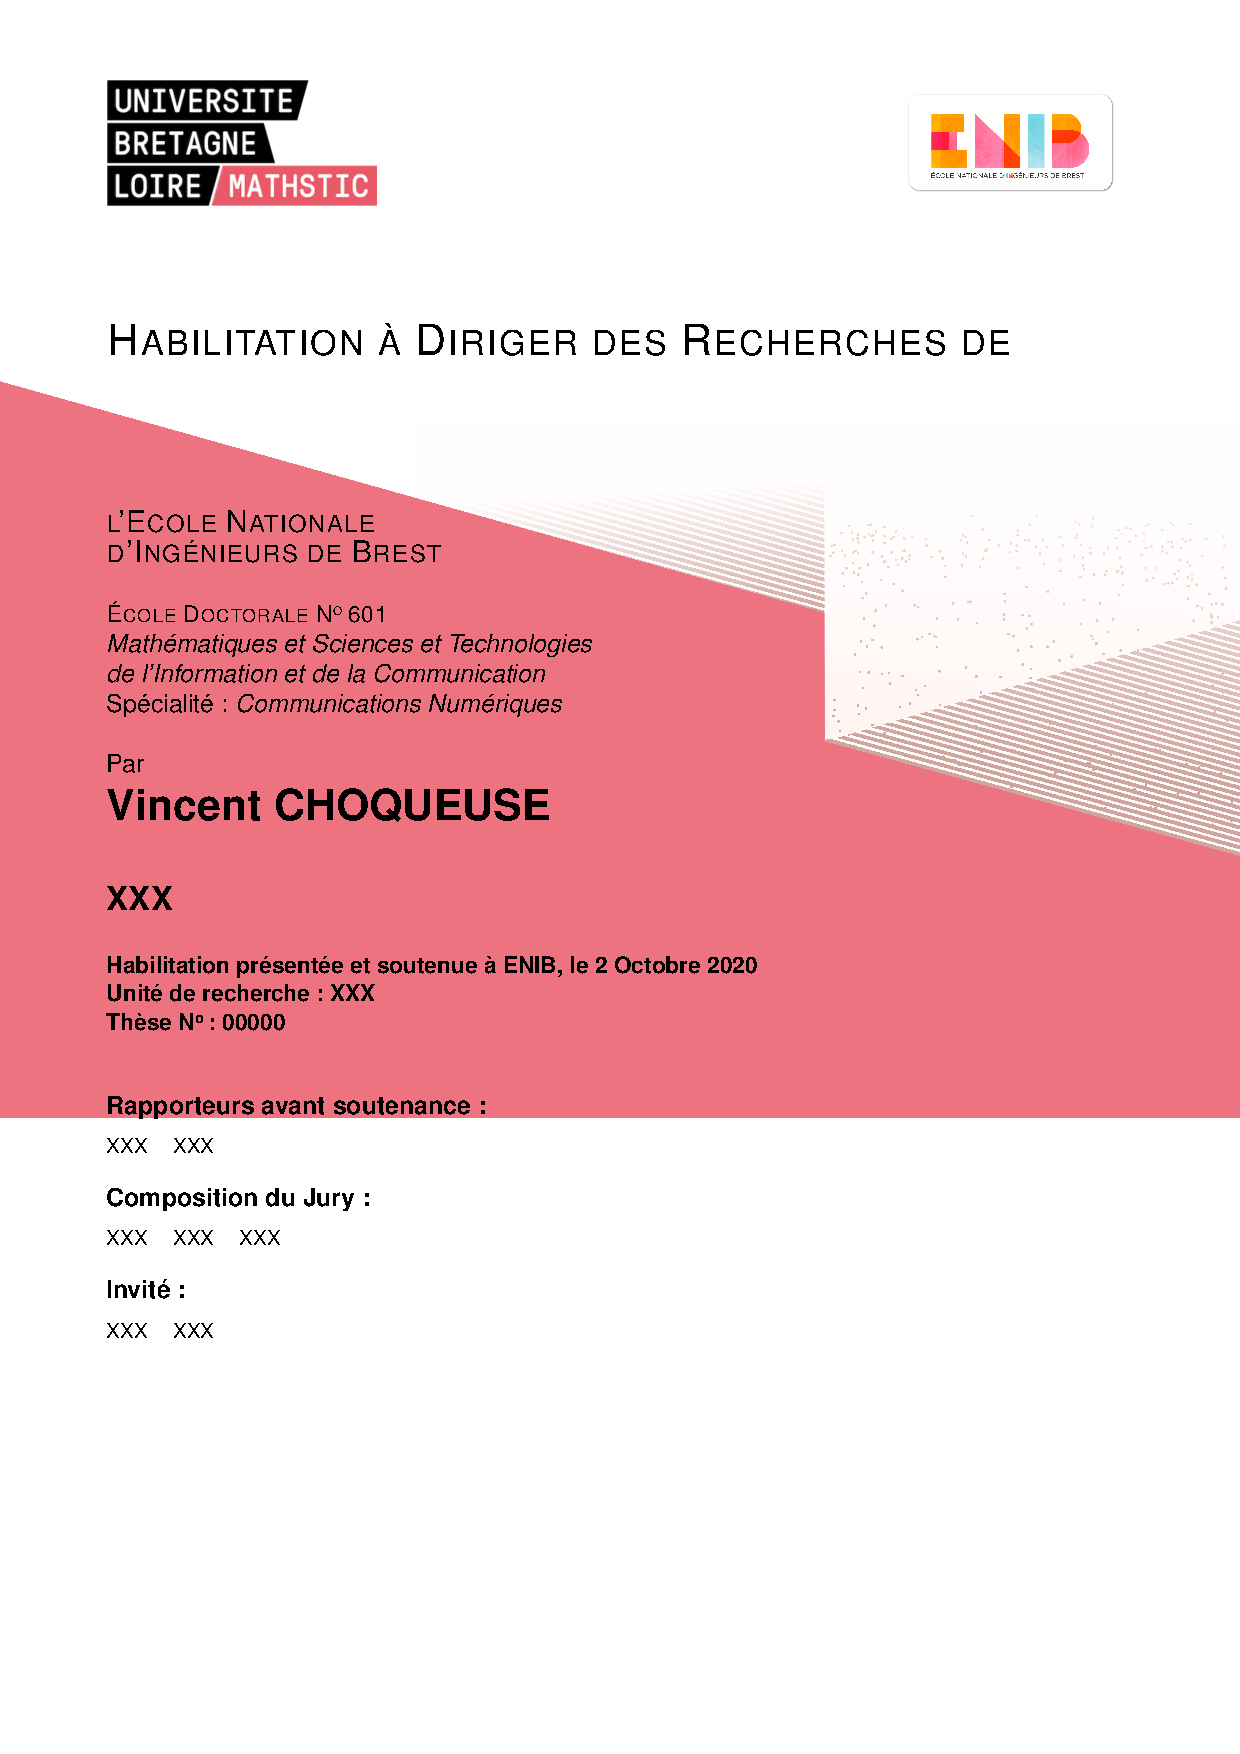
\includepdf[pages={1}]{cover/cover.pdf}

\newpage\null\thispagestyle{empty}\newpage
%\printnomenclature
\printglossary[type=acronym,title=Acronymes]
\cleardoublepage
\tableofcontents
\cleardoublepage
\pagenumbering{arabic}
\newpage
%newpage
%\listoffigures
%\newpage
%\listoftables
% !TEX root = ../HDR.tex

\chapter*{Remerciements}


% !TEX root = ../HDR.tex

\chapter*{Avant Propos}
\addcontentsline{toc}{chapter}{Avant Propos}  

\part{Volet Administratif}
% !TEX root =../HDR.tex



\chapter{Curriculum Vit\ae}
\label{chapCV}

\section{\'Etat Civil}

\begin{itemize}
\item \textbf{Nom, Prénom }: Choqueuse Vincent.
\item \textbf{Date et Lieu de Naissance }: né le 18 mai 1981 (39 ans) à Brest.
\item \textbf{Situation Familiale }: Pacsé, 2 enfants.
\item \textbf{Situation Professionnelle }: Maître de conférences en section 61 à l'\gls{enib}, \gls{labsticc} (UMR CNRS 6285).
\item \textbf{Site web }: \url{https://www.enib.fr/~choqueuse/}.
\item \textbf{Google Scholar}: \url{https://scholar.google.com/citations?user=nY4jZYQAAAAJ&hl=en} .
\item \textbf{Researchgate}: \url{https://www.researchgate.net/profile/Vincent_Choqueuse} .
\end{itemize}

\section{Parcours Académique}


\section{Activités Professionnelles}

\section{Responsabilités Collectives}


\section{Centres d'intérêt}

\chapter{Activités de Recherche}
\label{chapAR}

\section{Résumé des travaux de recherche}

\subsection{Maître de conférences à l'\gls{irdl}}
 

\subsection{Thèse de Doctorat}
\subsection{Stages de Master à Orange Labs, Lannion}

\section{Activité d'encadrement de jeunes chercheurs}

\subsection{Encadrement de thèses}

\subsection{Encadrement d'étudiants en Master}


\subsection{Participation à des jurys de thèses}

\section{Responsabilités administratives et collectives}

\section{Production Scientifique}

\part{Volet Recherche}
% !TEX root = ../HDR.tex

\chapter{Mon Chapitre 1}



\section{Introduction}

\subsection{Contexte}

\subsection{Problématique}

\section{Section 1}

\section{Section 2}

% !TEX root = ../HDR.tex

\chapter*{Conclusion Générale}
\addcontentsline{toc}{chapter}{Conclusion Générale}  


\cleardoublepage
\addcontentsline{toc}{chapter}{Bibliographie}
\bibliographystyle{acm} 
\bibliography{./bib/bibdesk.bib} 

\newpage\null\thispagestyle{empty}\newpage
\includepdf[pages={2}]{cover/cover.pdf}

\end{document}

